\subsection{Biological interpretation} \label{s:cs:bio_interp}

% Introduction our decision that we are going to use the work from Simon
The first part of the chapter established the clustering configuration, K-means with 5 groups, based on different clustering metrics. In this second part, the work is carried on understanding and establishing the biological aspects of the MIBC subtypes derived which involves comparing our classification with the others in the literature: TCGA \cite{Robertson2017-mg}, Lund \citet{Marzouka2018-ge} and the consensus \citet{Kamoun2020-tj}. It also requires Differentially Expressed Analysis (DEA) see \cref{da} and Gene Set Enrichment Analysis (GSEA) see \cref{asda} to establish the genes that contribute the most.


% TCGA and consensus classification
Comparing with the TCGA \citet{Robertson2017-mg} (and the consensus) it can be noticed in \cref{fig:cs:ifn_all} that the Ba/Sq is split into two a smaller and larger subgroups, there is a Neuroendocrine group (NE), a Luminal Papillary (LumP) group and a combine Luminal Infiltrated/Non-specified (Lum Inf/NS). 


\begin{figure}[!htb]
    \centering
    \begin{subfigure}[!t]{0.79\textwidth}
    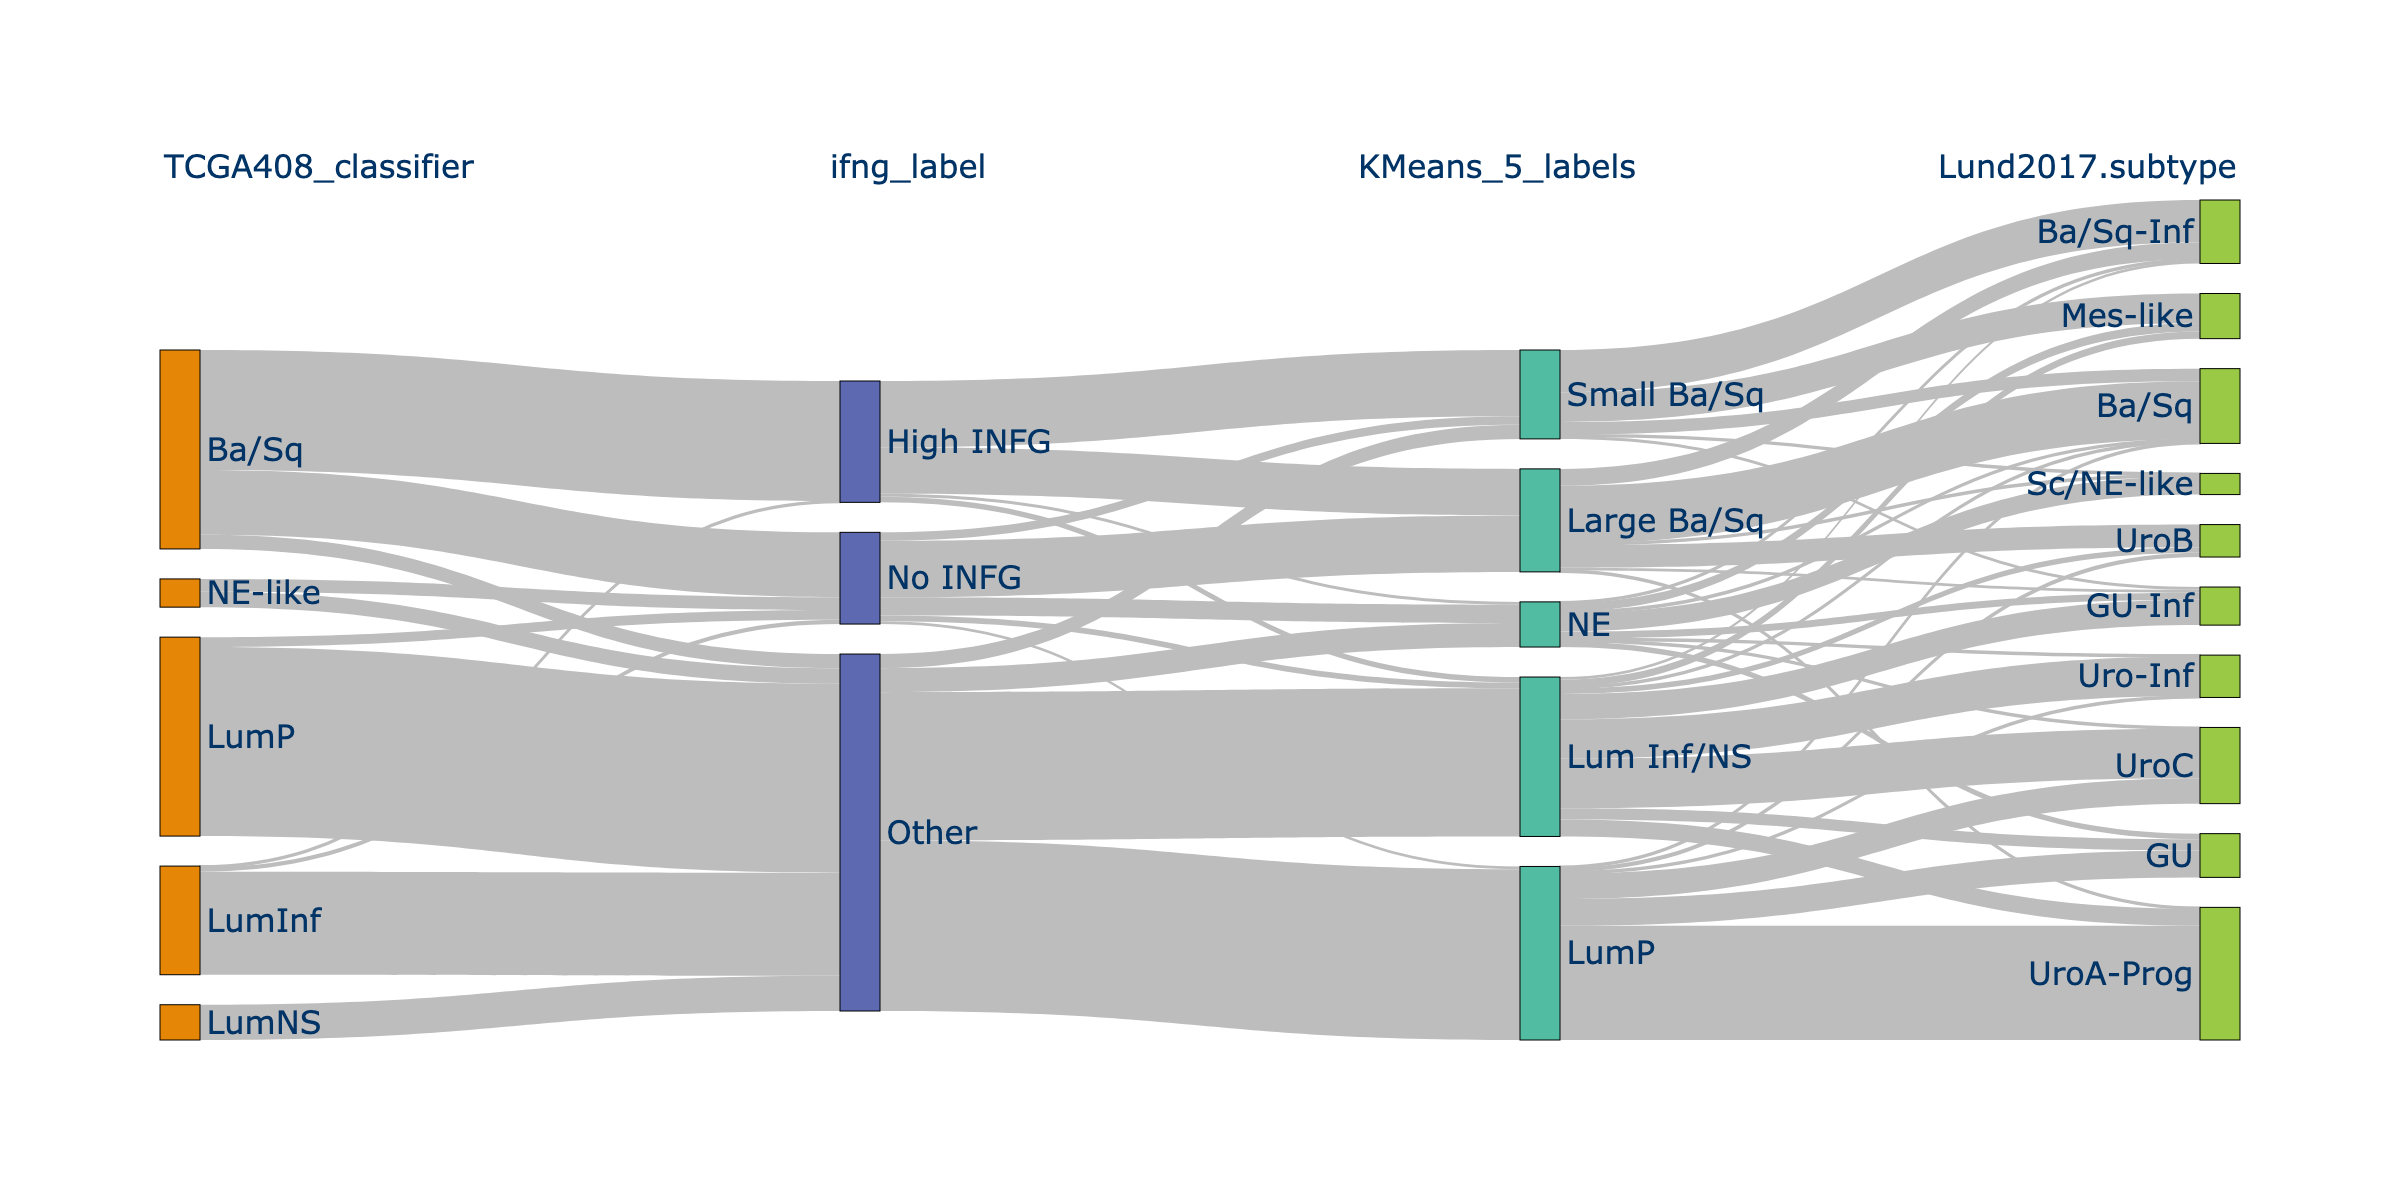
\includegraphics[width=1.0\textwidth,keepaspectratio]{Sections/ClusteringAnalysis/Resources/discussion/inf_comp.png}
        \caption{All the groups derived with K-means (K=5)}
        \label{fig:cs:ifn_all}
    \end{subfigure}
    \centering
    \begin{subfigure}[!t]{0.79\textwidth}
        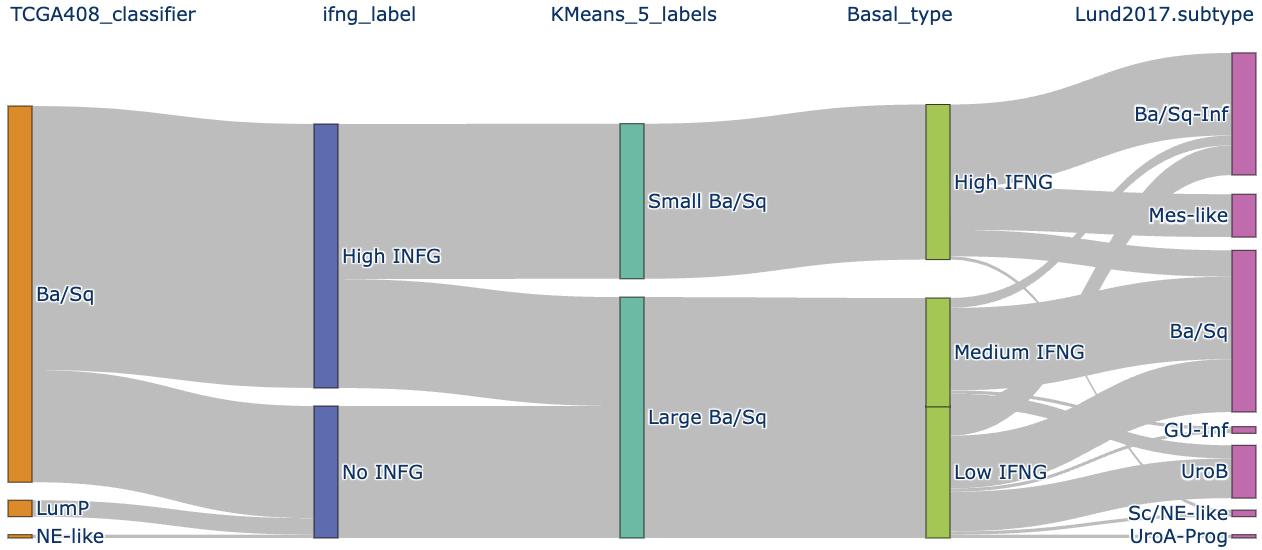
\includegraphics[width=\textwidth,keepaspectratio]{Sections/ClusteringAnalysis/Resources/discussion/inf_3_basal.png}
        \caption{Further split of the Basal group into 3 subtypes, using the work from \citet{Baker2022-bj}}
        \label{fig:cs:ifn_three_basal}
    \end{subfigure} 
    \centering
    \centering
    \caption{Sankey plot comparing the TCGA classification \citet{Robertson2017-mg}, the Interferon$\gamma$ split from \cite{Baker2022-bj}, our clustering and the Lund classifier \citet{Marzouka2018-ge}. This plot highlights that the two basal splits found through our clustering are a group of samples that have high \acrshort{ifn} (small group) and a mixed response (Large Ba/Sa). }
    \label{fig:cs:ifn_comp}
\end{figure}

% IFNG
The groups derived in this section are also compared with another work \citet{Baker2022-bj} from the Jack Birch Unit (JBU) which was focused on splitting the Basal/Squamous group by the tumour's \acrfull{ifn} response: no response and a high response. The authors identified that patients classified as high \acrshort{ifn} have a better survival prognosis compared to the ones with no immune response. In \cref{fig:cs:ifn_comp} it can be clearly seen that the Small Ba/Sq group contains a large portion of the the \acrshort{ifn} response group from \citet{Baker2022-bj}, while the large basal group a mixed of low and high \acrshort{ifn} samples. Taking the 3 main 'chords' of samples going from the \acrshort{ifn} to the Basal groups (KMeans), the Basal subtype can be further split into 3 as seen in \cref{fig:cs:ifn_three_basal}. The association of the Basal subgroups it is also supported by the Lund classifier \citet{Marzouka2018-ge}, where the Small Ba/sq (or High IFNG) contains the samples of the Ba/Sq-Inf and Mes-like from Lund, while the other two basal (in Basal\_type) are either Ba/Sq or UroB by Lund.

% Introduce the three splits
\paragraph*{Immune, Stromal and ESTIMATE score}

% Explaining the ESTIMATE score
In their seminal work, \citet{Yoshihara2013-wq} introduced the ESTIMATE score, which assesses tumour purity based on immune and stromal infiltration. The ESTIMATE score is calculated using gene expression data from a subset of genes that are known to be involved in the immune response and are associated with stromal cells. The ESTIMATE, along with stromal and immune scores, were validated using DNA Copy Number Analysis and computed for the TCGA cohort.

\begin{figure}[!htb]
    \centering
    \begin{subfigure}[!t]{0.49\textwidth}
        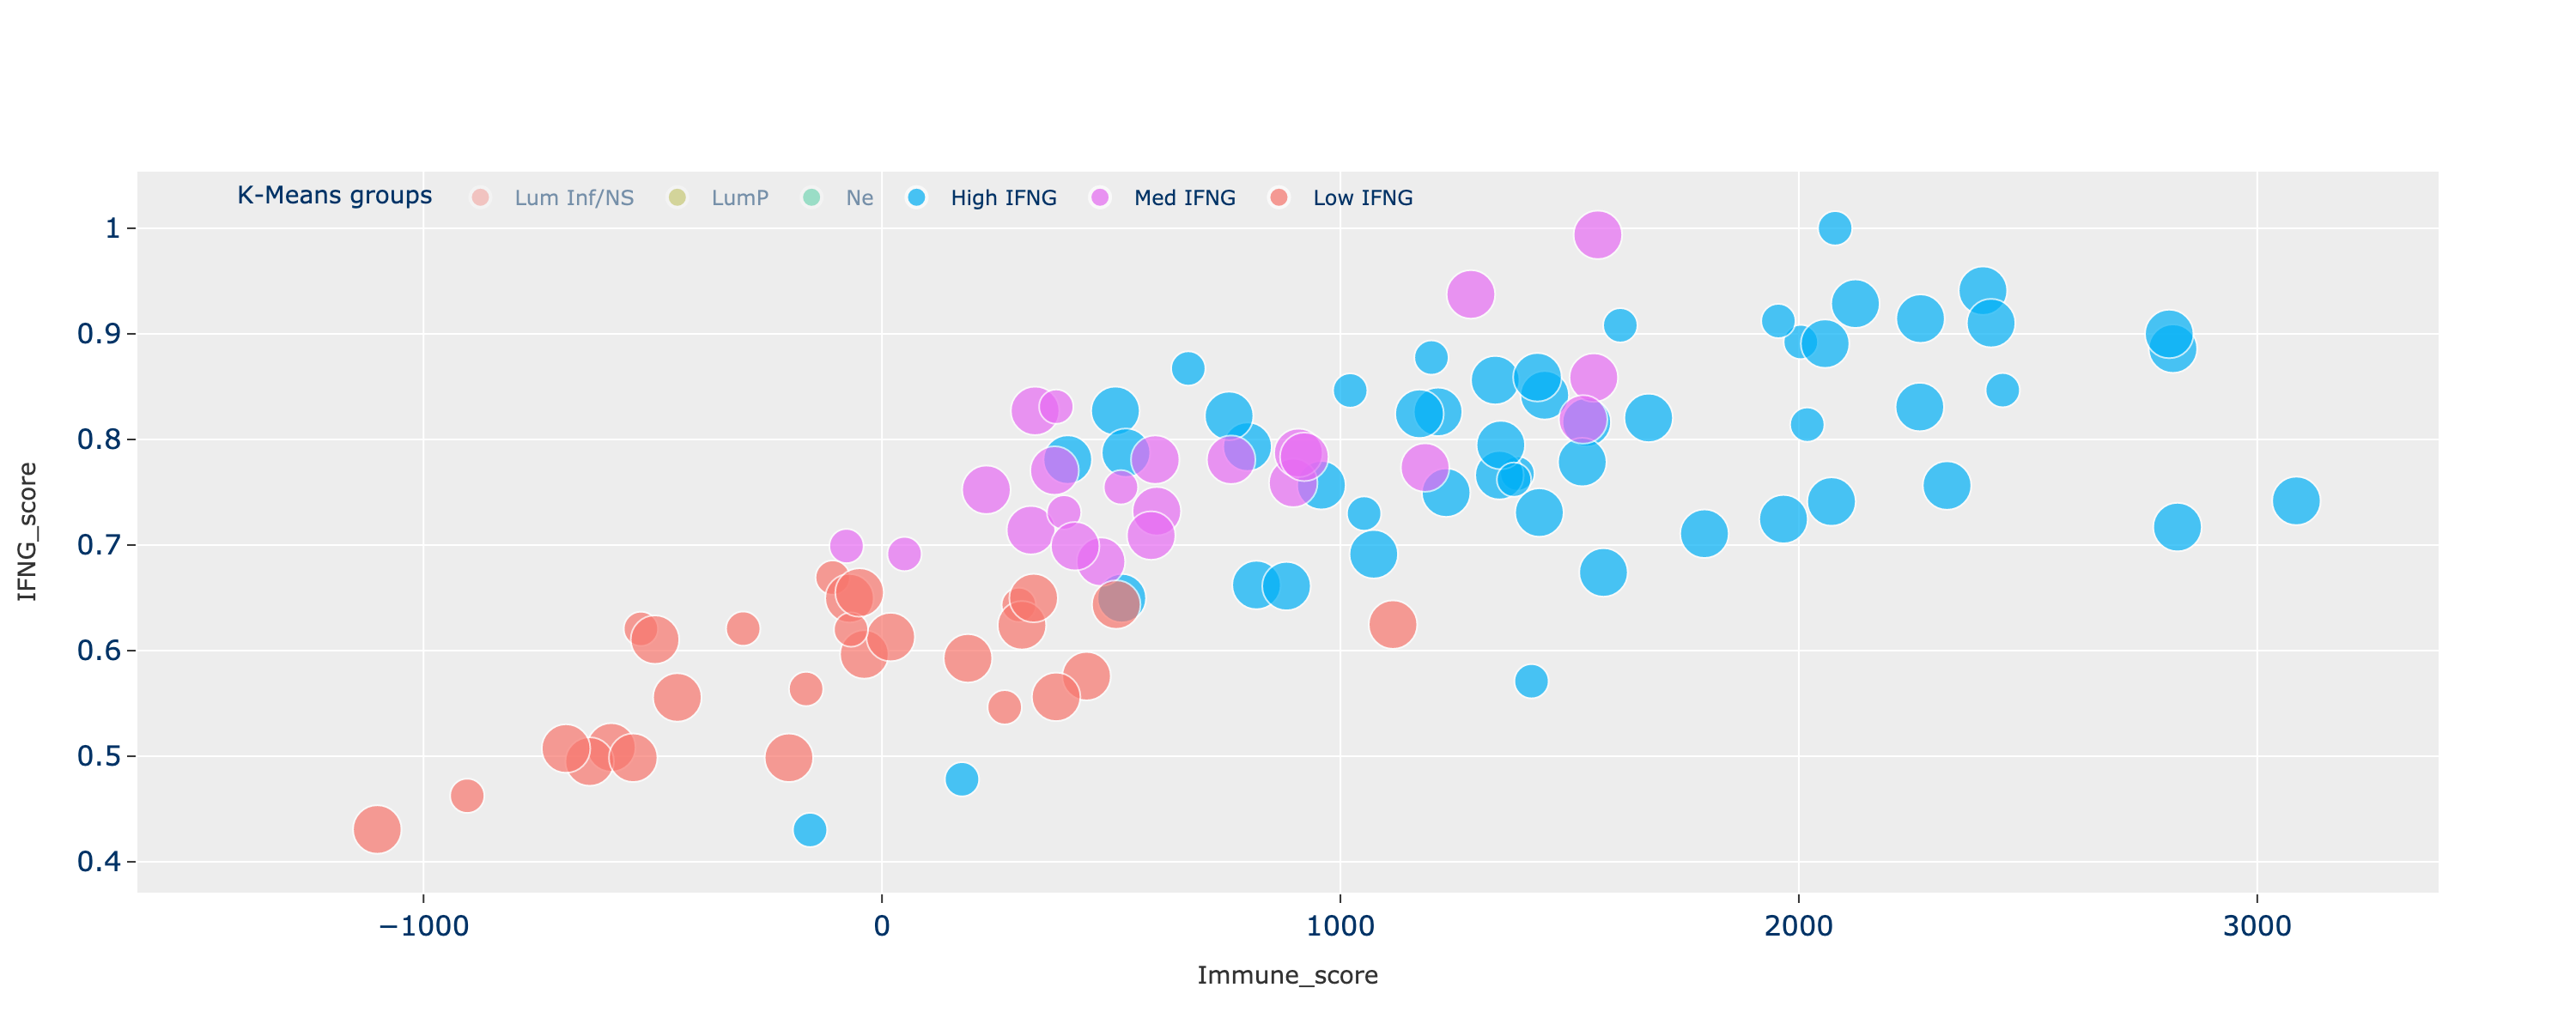
\includegraphics[width=\textwidth,keepaspectratio]{Sections/ClusteringAnalysis/Resources/discussion/Immune_spectrum.png}    
        \caption{Immune Score}
        \label{fig:cs:immune_basal}
    \end{subfigure}
    \centering
    \begin{subfigure}[!t]{0.49\textwidth}
        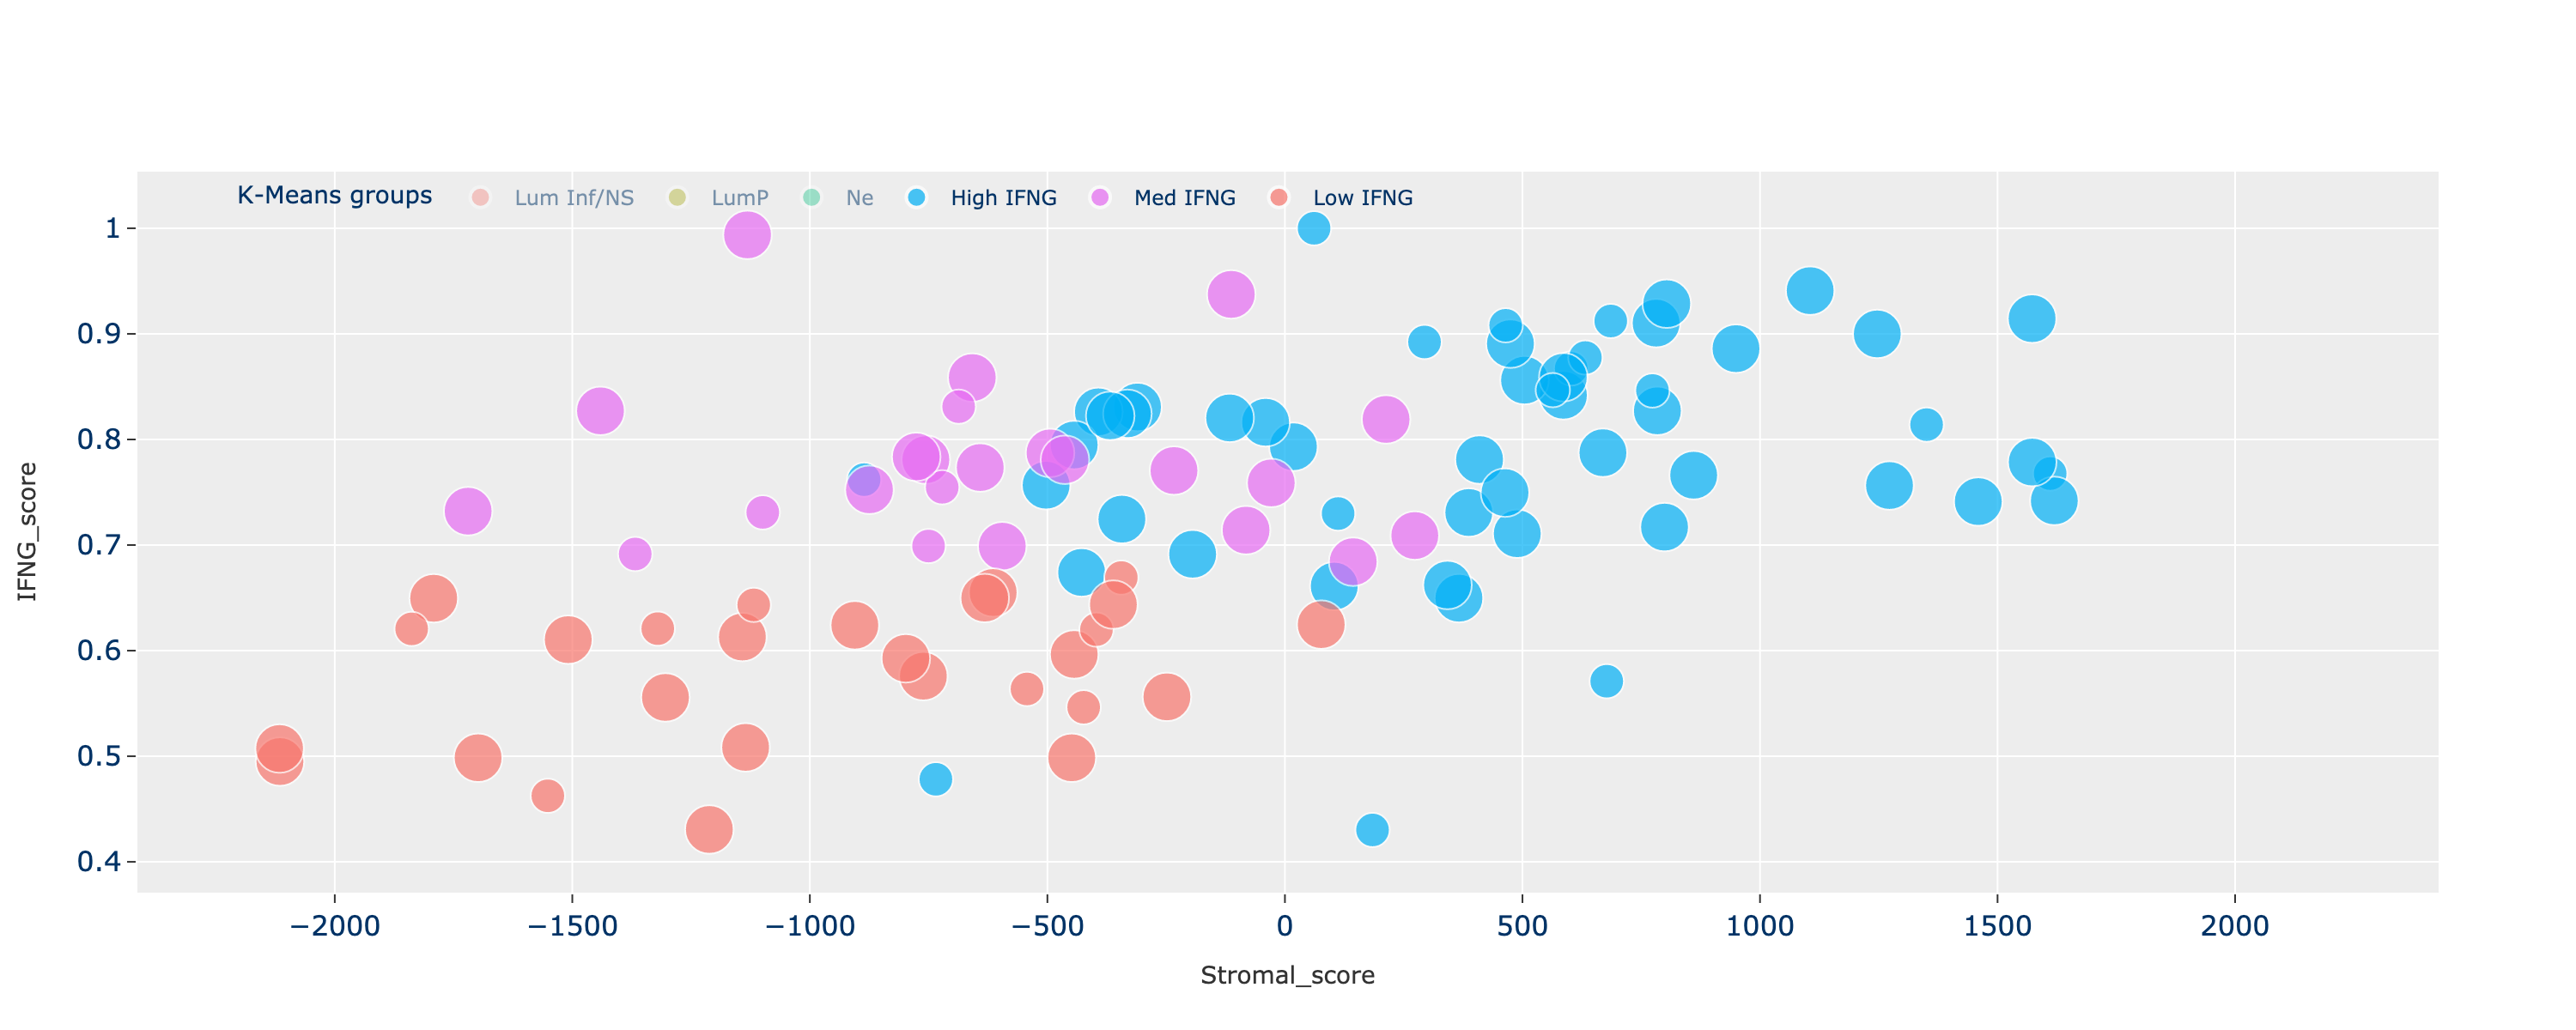
\includegraphics[width=\textwidth,keepaspectratio]{Sections/ClusteringAnalysis/Resources/discussion/Stroma_spectrum.png}
        \caption{Stroma Score}
        \label{fig:cs:stroma_basal}
    \end{subfigure} 
    \centering
    \begin{subfigure}[!t]{0.7\textwidth}
        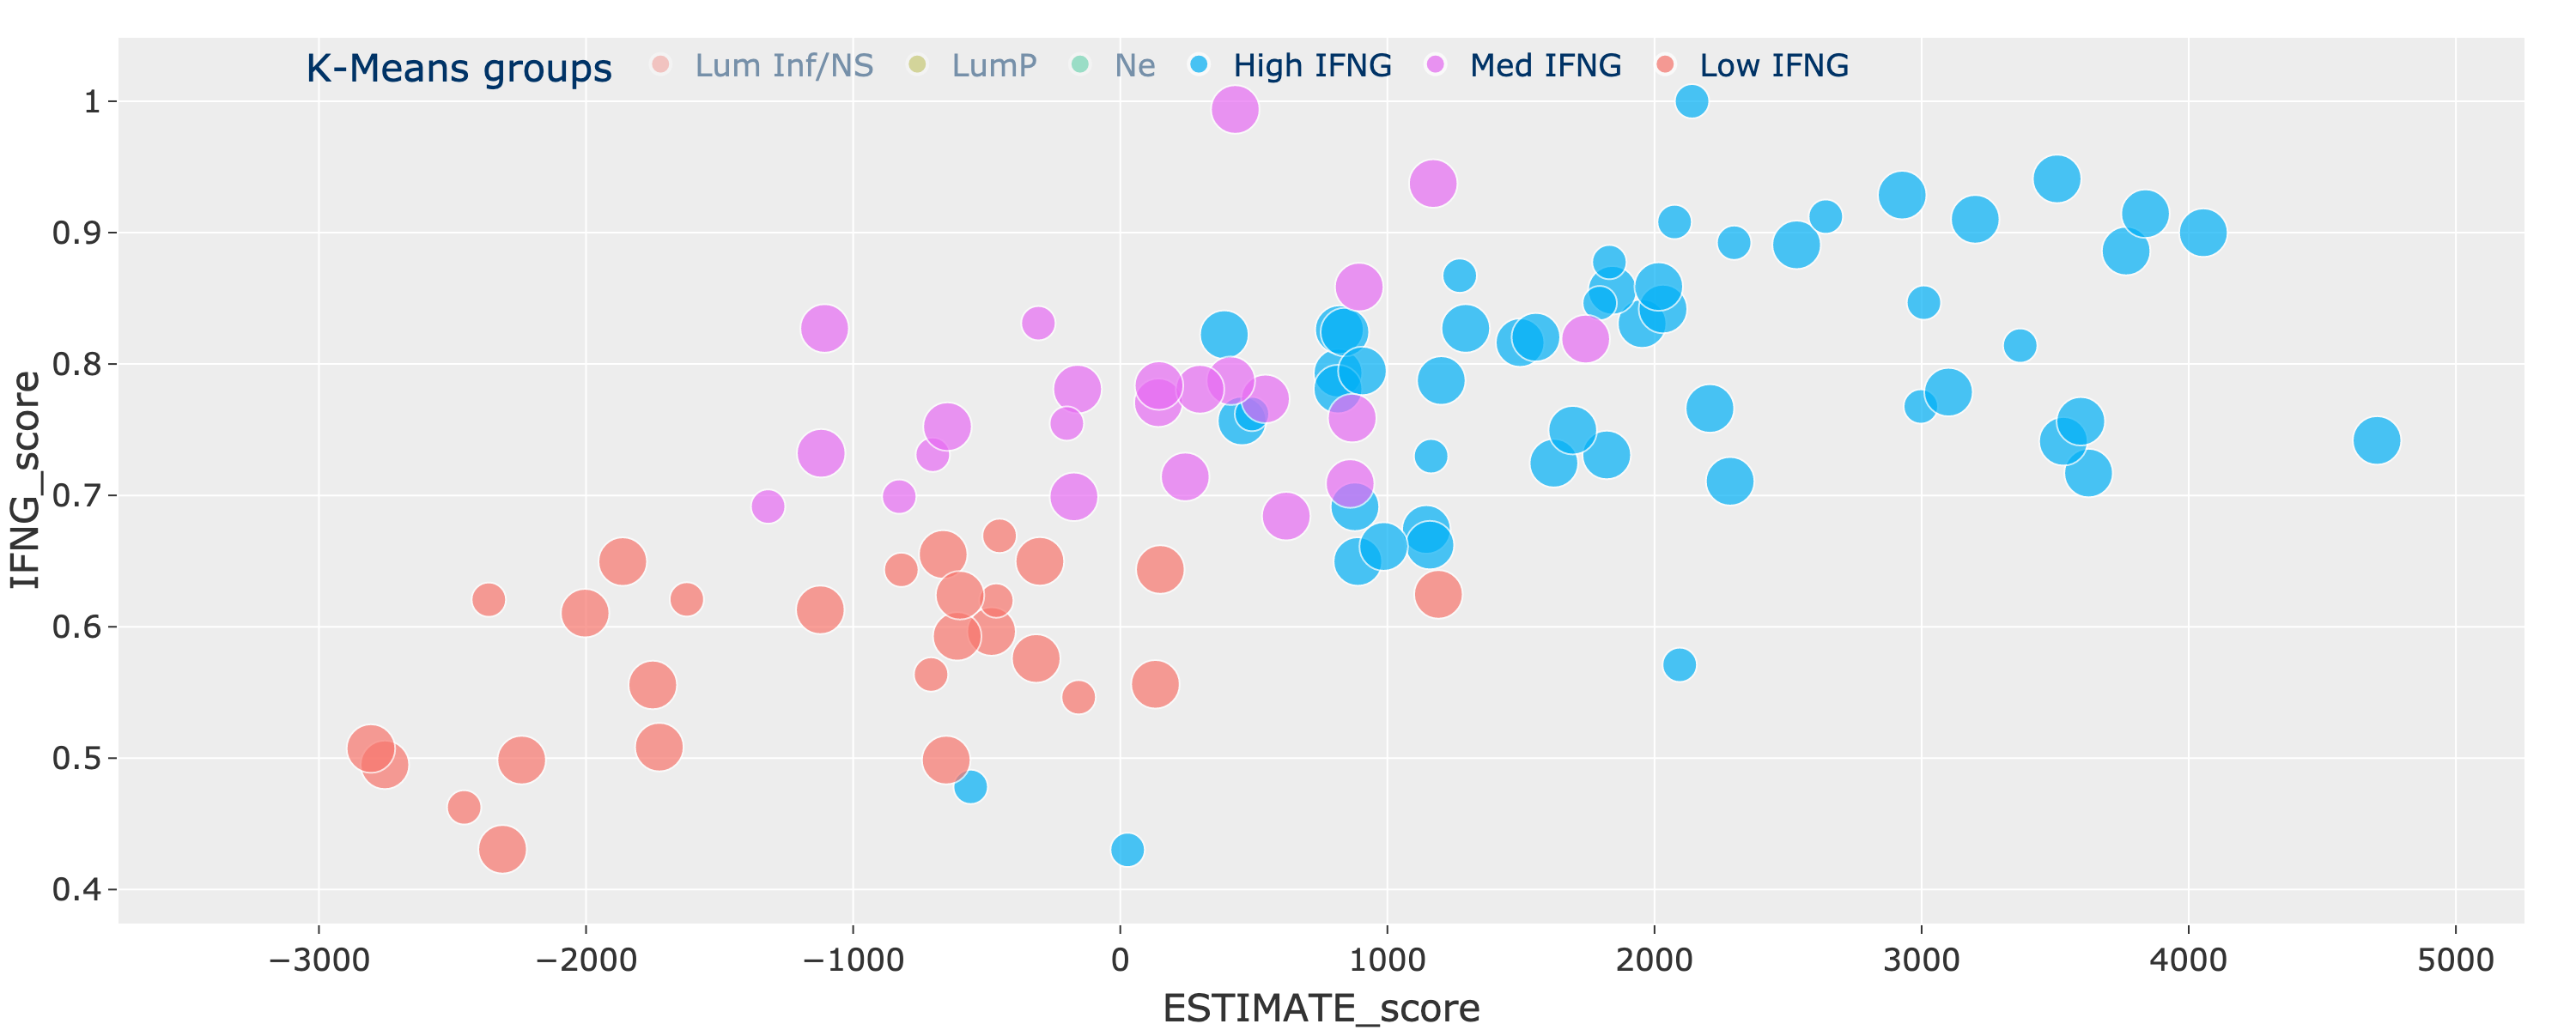
\includegraphics[width=\textwidth,keepaspectratio]{Sections/ClusteringAnalysis/Resources/discussion/Estimate_spectrum.png}
        \caption{ESTIMATE}
        \label{fig:cs:estimate_basal}
    \end{subfigure}
    \centering
    \caption{The tumour purity as indicated by the immune, stroma, and ESTIMATE scores from \citet{Yoshihara2013-wq} for the three basal splits. In all scatter plots, the Y-axis is represented by the \acrshort{ifn} score from \citet{Baker2022-bj}, the X-axis by one of the three scores, and the size of the markers is proportional to the infiltration score from \citet{Robertson2017-mg}. Positive values of the score denote infiltration by the type of cells, while negative values indicate their absence.}
    \label{fig:cs:tumour_purity}
\end{figure}


% Check the three splits along the immune infiltration, ESTIMATE, and stroma score
The three Basal/Squamous splits, using both K-means with \( K = 5 \) and the work of \acrshort{ifn} response, can be classified into three different levels of immune response: Low, Medium, and High \acrshort{ifn} response, as seen in \cref{fig:cs:ifn_three_basal}. Across all the plots, the Y-axis is represented by the \acrshort{ifn} score from \citet{Baker2022-bj}, and the X-axis represents one of the three scores from \citet{Yoshihara2013-wq}, while the scatter plot is represented by the infiltration score from the TCGA's metadata. The first scatter plot shows that High \acrshort{ifn} has the largest immune infiltration and \acrshort{ifn} response, while Low \acrshort{ifn} is at the opposite end of the spectrum, with Medium \acrshort{ifn} somewhere in between. This plot further strengthens the relationship between the Basal splits and the immune response.

\Cref{fig:cs:stroma_basal} shows the relationship between the three Basal subgroups and stromal infiltration. The spectrum is not as clear as in the previous plot, as both Low and Medium \acrshort{ifn} have a low stromal score, but the differences with the other Basal groups are clear. Lastly, the two scores are combined in the ESTIMATE scatter plot, shown in \cref{fig:cs:estimate_basal}, displaying the tumour purity of the samples in the three groups. The figure illustrates the spectrum-like nature of the Basal subtypes and their relationship, with Low \acrshort{ifn} showing the highest purity, followed by Medium and High \acrshort{ifn}, the latter being the most impure for stromal cell and immune infiltration. 


The scores from \citet{Yoshihara2013-wq} further support their relation with the immune, stromal and tumour purity. In the previous work which split the Basal group into two based on the immune response, Lund classifier \citet{Marzouka2018-ge} and \acrshort{ifn} response from \citet{Baker2022-bj}, the groups with the higher response also had a better survival prognosis. This is further supported by the Kaplan-Meier survival analysis shown in \cref{fig:cs:basal_survival} where the Basal group from \citet{Robertson2017-mg} is shown by the green line, where the other 3 lines are represented by the subtypes derived in this section. From the survival rates it can be noticed how the 3 basal groups constitute the TCGA's Ba/Sq group and the poorer prognosis for the Low IFNG samples. This plot shows the importance of improving the MIBC classifications. 

\begin{figure}[!htb]    
    \centering
    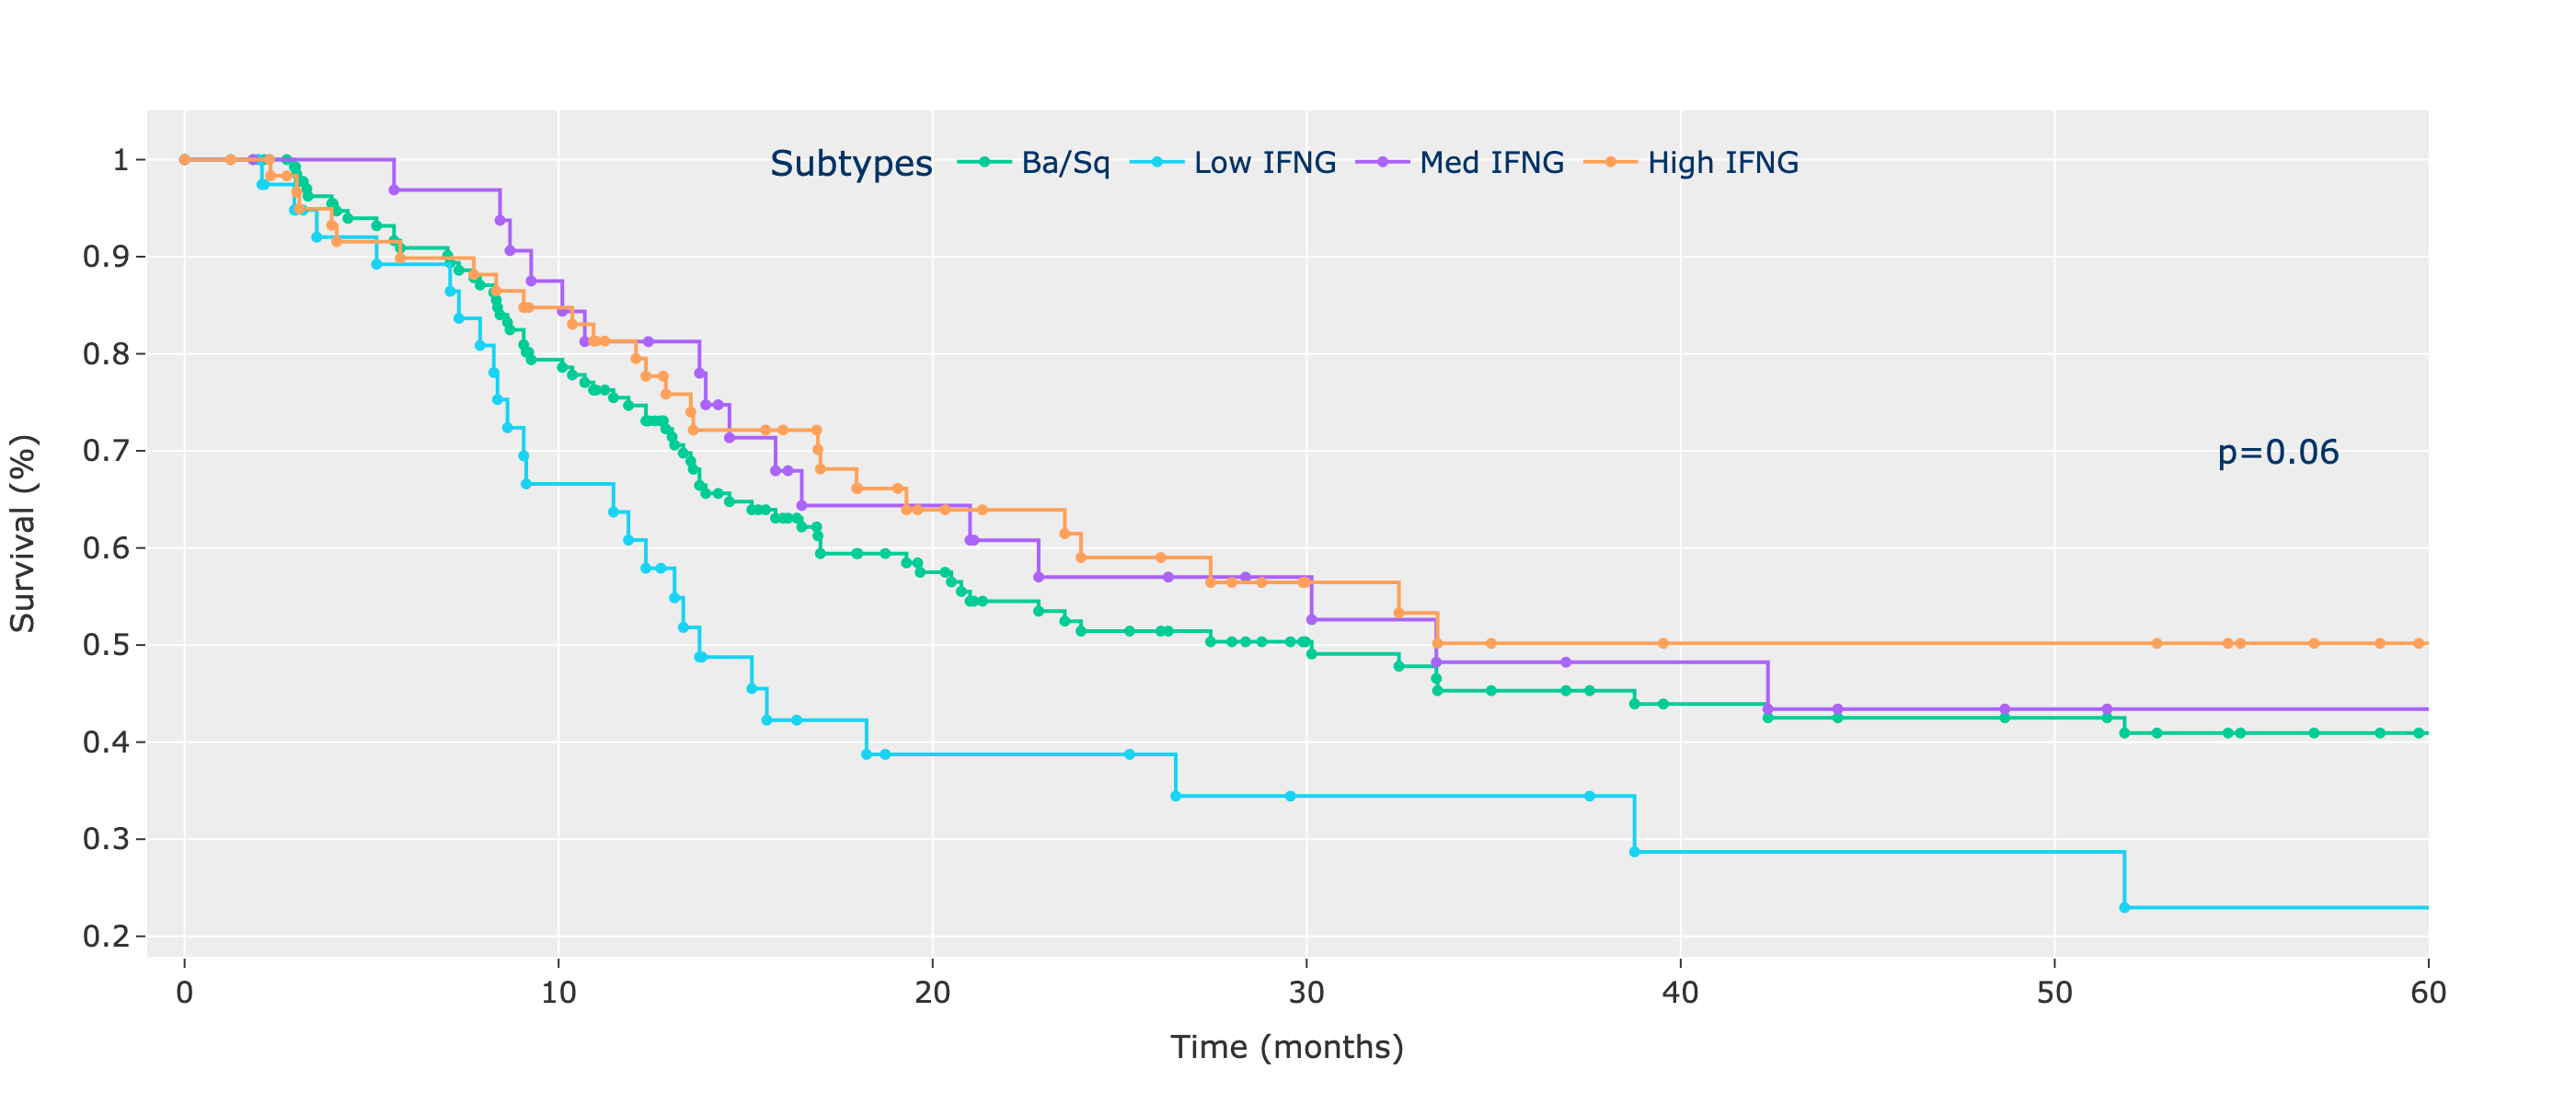
\includegraphics[width=1.0\textwidth,keepaspectratio]{Sections/ClusteringAnalysis/Resources/discussion/survival_basal.png}
    \caption{Kaplan-Meier survival analysis of the 3 Basal groups derived in \cref{s:cs:bio_interp} using K-means with K=5 and the basal subgroups by the \acrshort{ifn} response \citet{Baker2022-bj}, and the Ba/Sq survival from TCGA classification \citet{Robertson2017-mg}.}
    \label{fig:cs:basal_survival}
\end{figure}

\paragraph*{Differentially Expressed Analysis}

To further study the subgroups derived, Deferentially Expressed Analysis (DEA) was performed between the MIBC subtypes. The analysis was particularly focused on the Basal groups as the three split was new with some already validated results through other classifications \citet{Baker2022-bj,Marzouka2018-ge}. The Pi-plot in \cref{fig:cs:pi_basal} compares the Low IFNG with the MED IFNG on the Y-axis and the Low IFNG with the High IFNG on the X-axis. 

% Low IFNG
The first thing to notice in the scatter plot is the small number of markers on the quadrant where the genes specific to Low IFNG are. This means, that there are not many genes that are differentiate the Low IFNG over the other Basal subtypes. On the X-axis, highlighting the points specific of the low IFNG over the High IFNG, there are many genes known as squamous markers such as \textit{ZBTB7C, TP64, DSC3}. Interestingly \textit{FGFR3} which is a known differentiated-associated marker and well-studied gene in MIBC is also on the X-axis. 

\begin{figure}[!htb]    
    \centering
    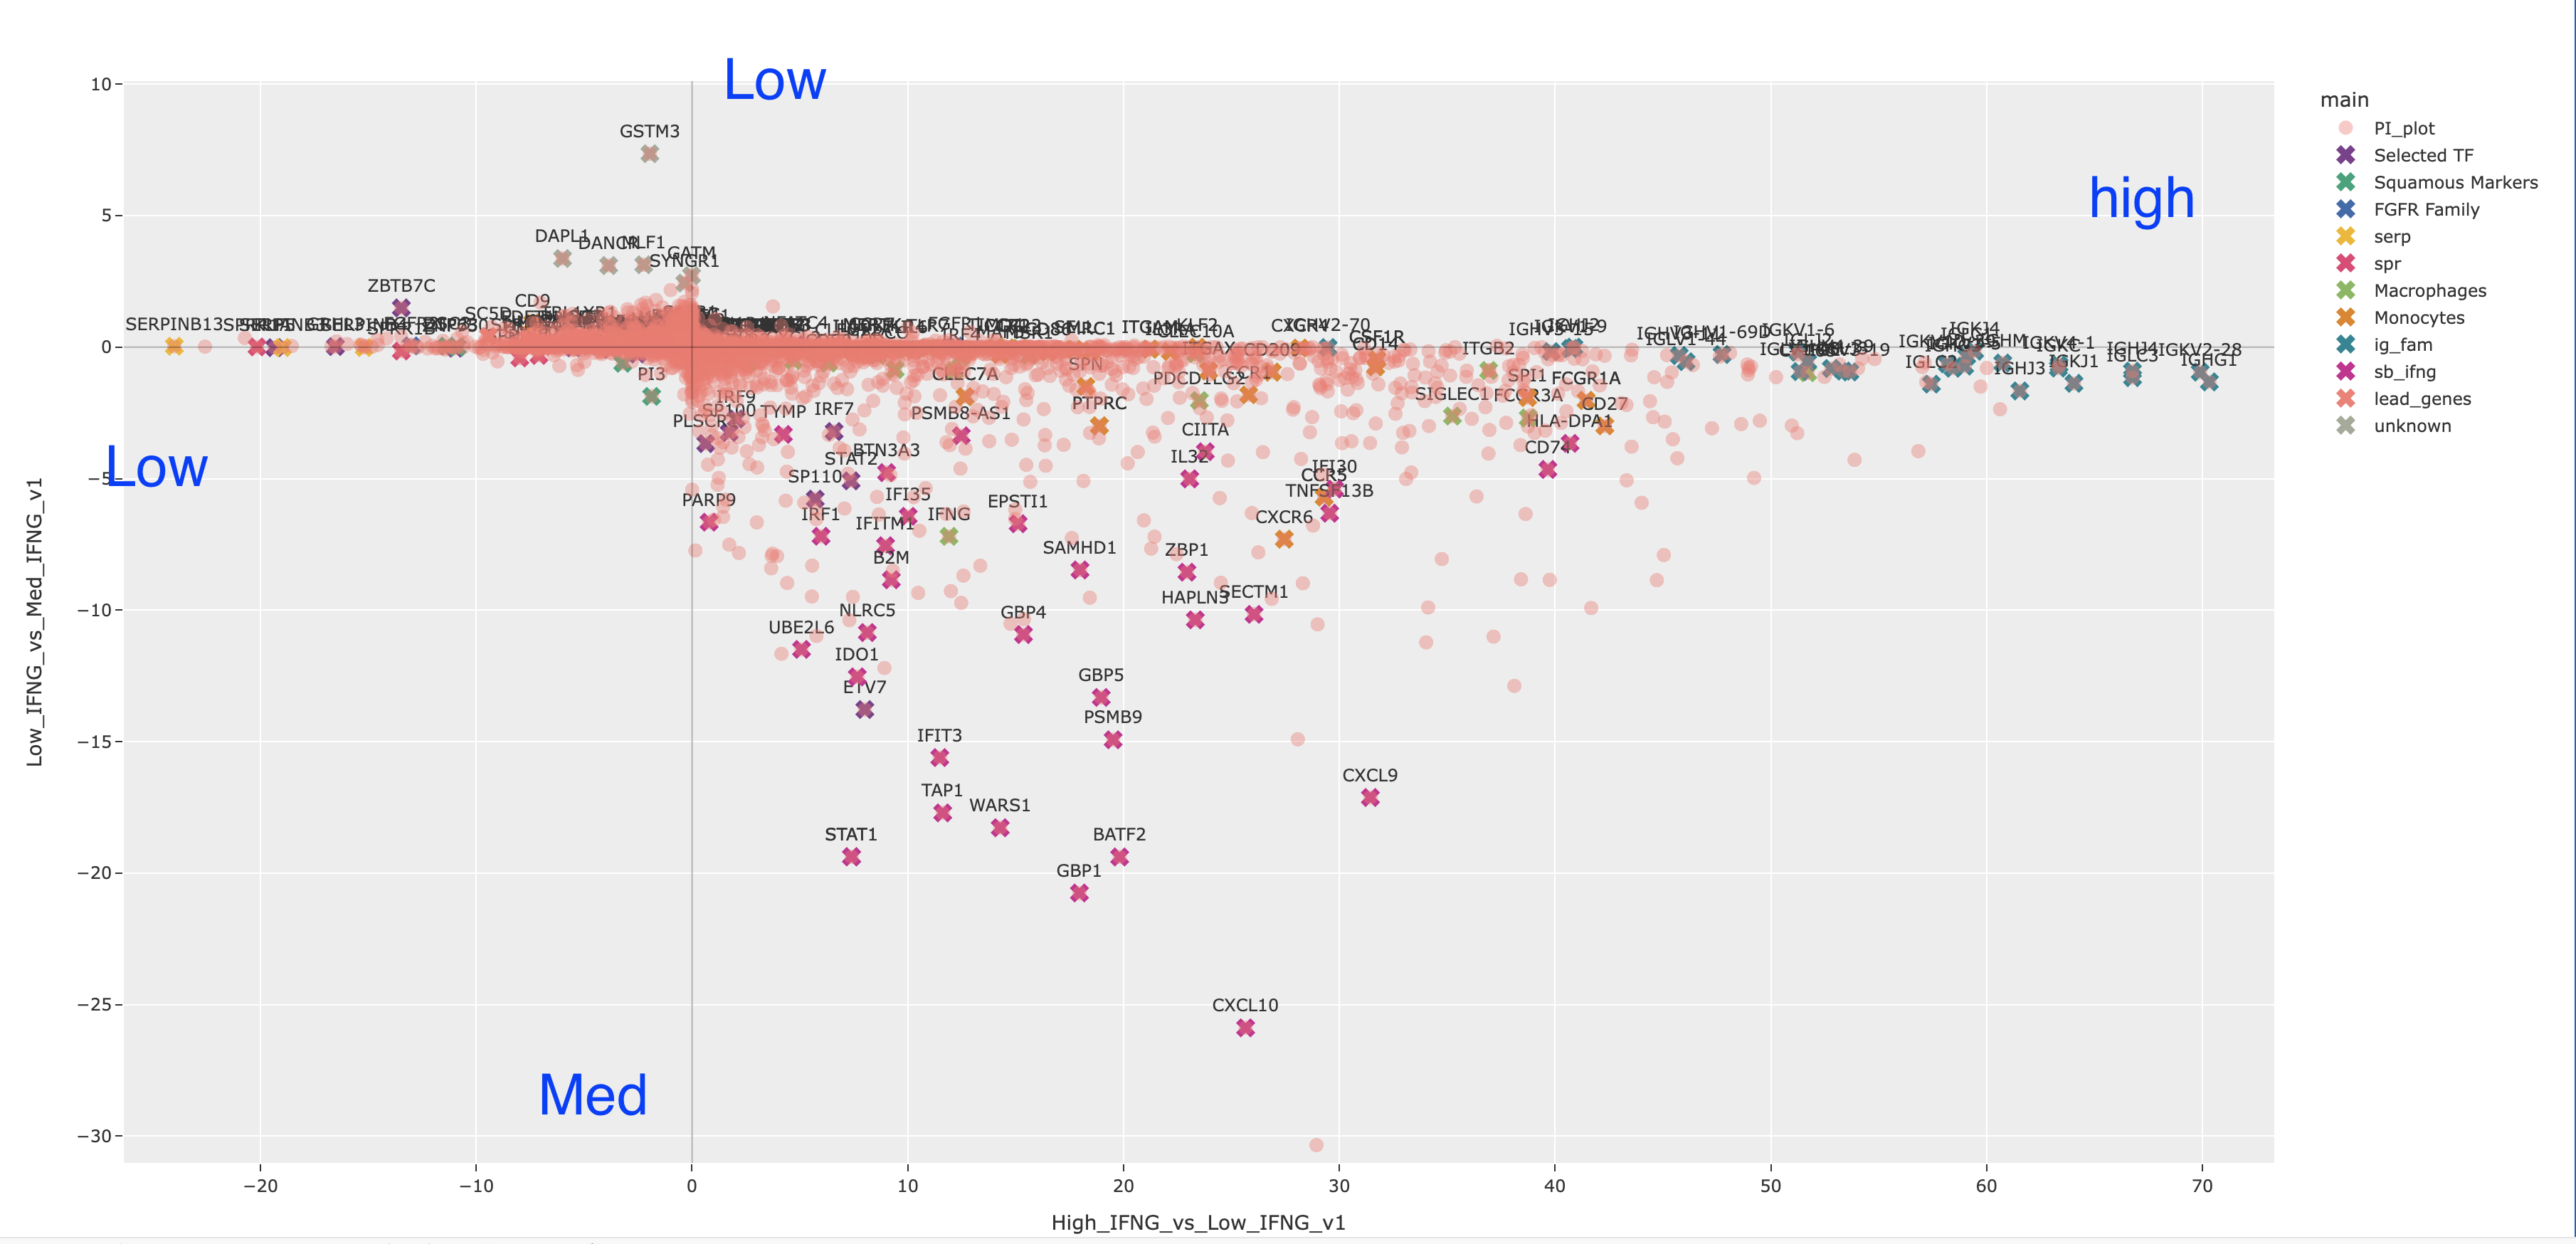
\includegraphics[width=1.0\textwidth,keepaspectratio]{Sections/ClusteringAnalysis/Resources/discussion/low_basal.png}
    \caption{Pi plot showing the two DEA run, on the X-axis: the Low vs High IFNG and on the Y-axis: the Low vs Med IFNG. }
    \label{fig:cs:pi_basal}
\end{figure}

Some of the genes, \textit{DANCR, DAPL1, GATM, GSTM3, MLF1, SYNGR1, GSTM1, MAGI3}, on the positive side of the Y-axis labelled as 'other' were not classified by any of the 'known markers'. However, some of them have a role in bladder or other cancers. In the work of \citet{Zhan2018-um} it was found that \textit{DANCR} (or \textit{ANCR}) is a long non-coding RNA (lncRNA) found to play an oncogenic role in bladder cancer\footnote{There is a review from \citet{Wang2021-gn} on the role of \textit{DANCR} in bladder and other cancers.}. According to \citet{Li2023-mk}, \textit{MLF1} might be involved in cancer, including bladder cancer and may influence the immune response. \textit{GATM} has the potential to be a tumour suppressor gene and influence a type of metastatic renal cancer \citet{Jee2022-wi}. \textit{GSTM3} along \textit{GSTM3} are known to be genetic risk factors for bladder cancer \citet{Schnakenberg2000-cu}. The role of \textit{MAGI3, MLF1, DAPL1} is less known.

% High IFNG and MEDIUM 
On the diagonally opposite quadrant are the genes involved in both High and Medium IFNG Basal groups which contains considerably more markers than the Low IFNG's quadrant. On the positive x-axis  most of the genes are part of the Immunoglobulin family (\textit{IG-}), genes associated with Macrophages, Monocytes all known to be related with the immune response. This confirms that the High IFNG is the strongest Basal subgroup associated with the immune response. The \acrshort{ifn} response markers from \citet{Baker2022-bj} are enriched in both Med and High IFNG subtypes as it is shown by the purple markers.


% Introduce the other plot
To further investigate the relationship of the Basal groups with the immune response of the tissue, another Pi plot was used in \cref{fig:cs:pi_basal_inf}. There Y axis has the Pi values generated from the DEA of Low IFNG vs Luminal Infiltrated, while the X-axis the DEA is between High and Med IFNG subgroups. In this case the Low IFNG is used as the MIBC subtype with least immune response while the Lum INF as non-basal group with high immune infiltration. Then, this scatter plot allows to the tendencies of the three Basal subtypes.

% High IFNG
The first quadrant contains he markers that are specific to both the LumInf and the High IFNG groups. It can be seen that the family of genes for immunoglobulin are common to both groups, but with a tendency for the High IFNG. On the positive X-axis there are many markers for other immune related response such as B, T cells as well as Monocites or Macrophages. This further reinforce the immune characteristics seen earlier for the High IFNG. It also shows how much of a stronger response the High IFNG has over the Med IFNG.

\begin{figure}[!htb]    
    \centering
    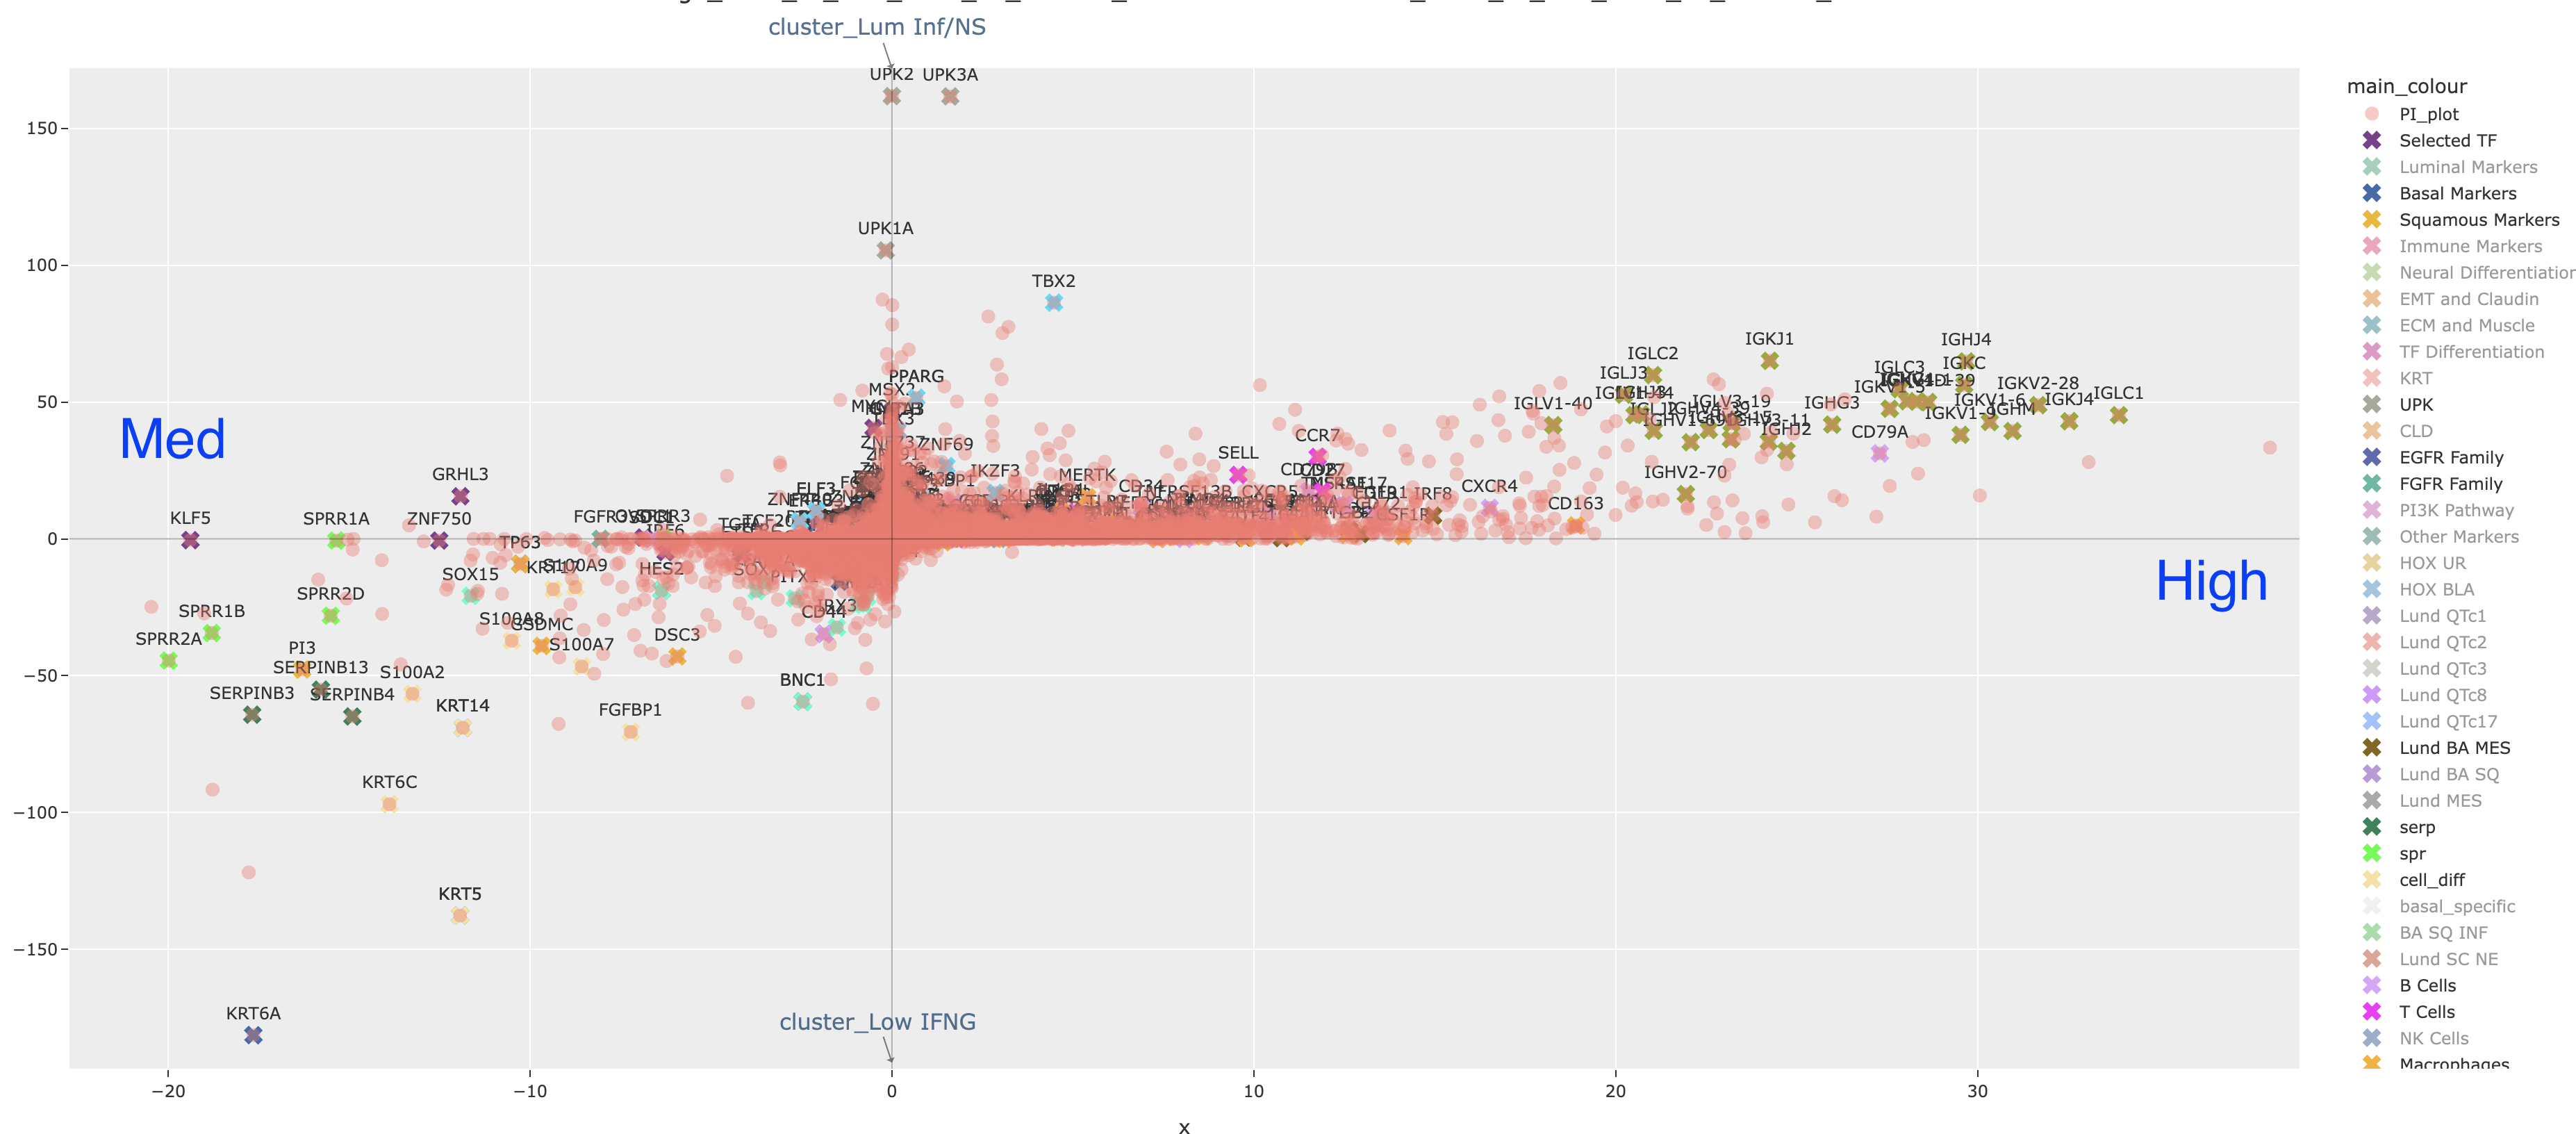
\includegraphics[width=1.0\textwidth,keepaspectratio]{Sections/ClusteringAnalysis/Resources/discussion/basal_infiltrated.png}
    \caption{Pi plot showing the two DEA run, on the X-axis: the Med vs High IFNG and on the Y-axis: the Luminal Infiltrated vs Low IFNG. }
    \label{fig:cs:pi_basal_inf}
\end{figure}


% Medium and LumInf
It can be noticed less common genes between the Med IFNG and the LumInf, in the forth quadrant. Some of the genes on the negative side of the Y-axis, which are specific to Med IFNG over the High IFNG are genes involved in the squamous or basal tissue such as \textit{ZBTB7C, ZNF750, KRT13, \textbf{KLF5}, SPRR1A}. The genes specific to Ba/Sq are even more present in the third quadrant, between the Low and Med IFNG, where many of the common genes are well know squamous or basal markers: \textit{DSC3, KRT6A, KRT5, TP63}, the \textit{SERPIN} and \textit{SPR} families.


The two figures \cref{fig:cs:pi_basal,fig:cs:pi_basal_inf} further reinforce the existence of the three different immune response by the basal tumours. It shows the genes specific to each of the subtypes, where the High IFNG has very specific immune responses even compared to the LumInf subgroup. The Med IFNG is situated somewhere between a high immune response and no response as seen in the samples from Low IFNG. Basal and Squamous markers are seen in both Low and Med IFNG groups as clearly seen in \cref{fig:cs:pi_basal_inf}, which also have been supported by the ESTIMATE scores \cref{fig:cs:tumour_purity}.





% Immune response on the other quadrant



% Then do the Survial plot and the Sankey to show the final version


\subsubsection{Summary}

The key finding in that by tweaking the gene filtering process and using a simple clustering approach, it was found that the canonical Basal group can be split into two based on the immune response. This shows that even without additional data such as immunochemistry or in-vitro experiments, new subgroups are yet to found with a biological importance.

This is not to say that the additional data does not improve the classification, but the contrary as the Basal group was further divided into three subgroups, one with a much lower survival prognosis. 

% The Basal split into two subgroups is not new, as it was shown in the Lund classification \citet{Marzouka2018-ge} and in-vitro experiments on \acrshort{ifn} from \citet{Baker2022-bj}. In both cases the group with a better immune response had a better survival prognosis.

% Previously, in the Lund classification \citet{Marzouka2018-ge} and in-vitro experiments on \acrshort{ifn} from \citet{Baker2022-bj}, it was shown that the Basal can be split into two. In both cases the group with a better immune response had a better survival prognosis.

\begin{figure}[!htb]
    \centering
    \begin{subfigure}[!t]{1.0\textwidth}
        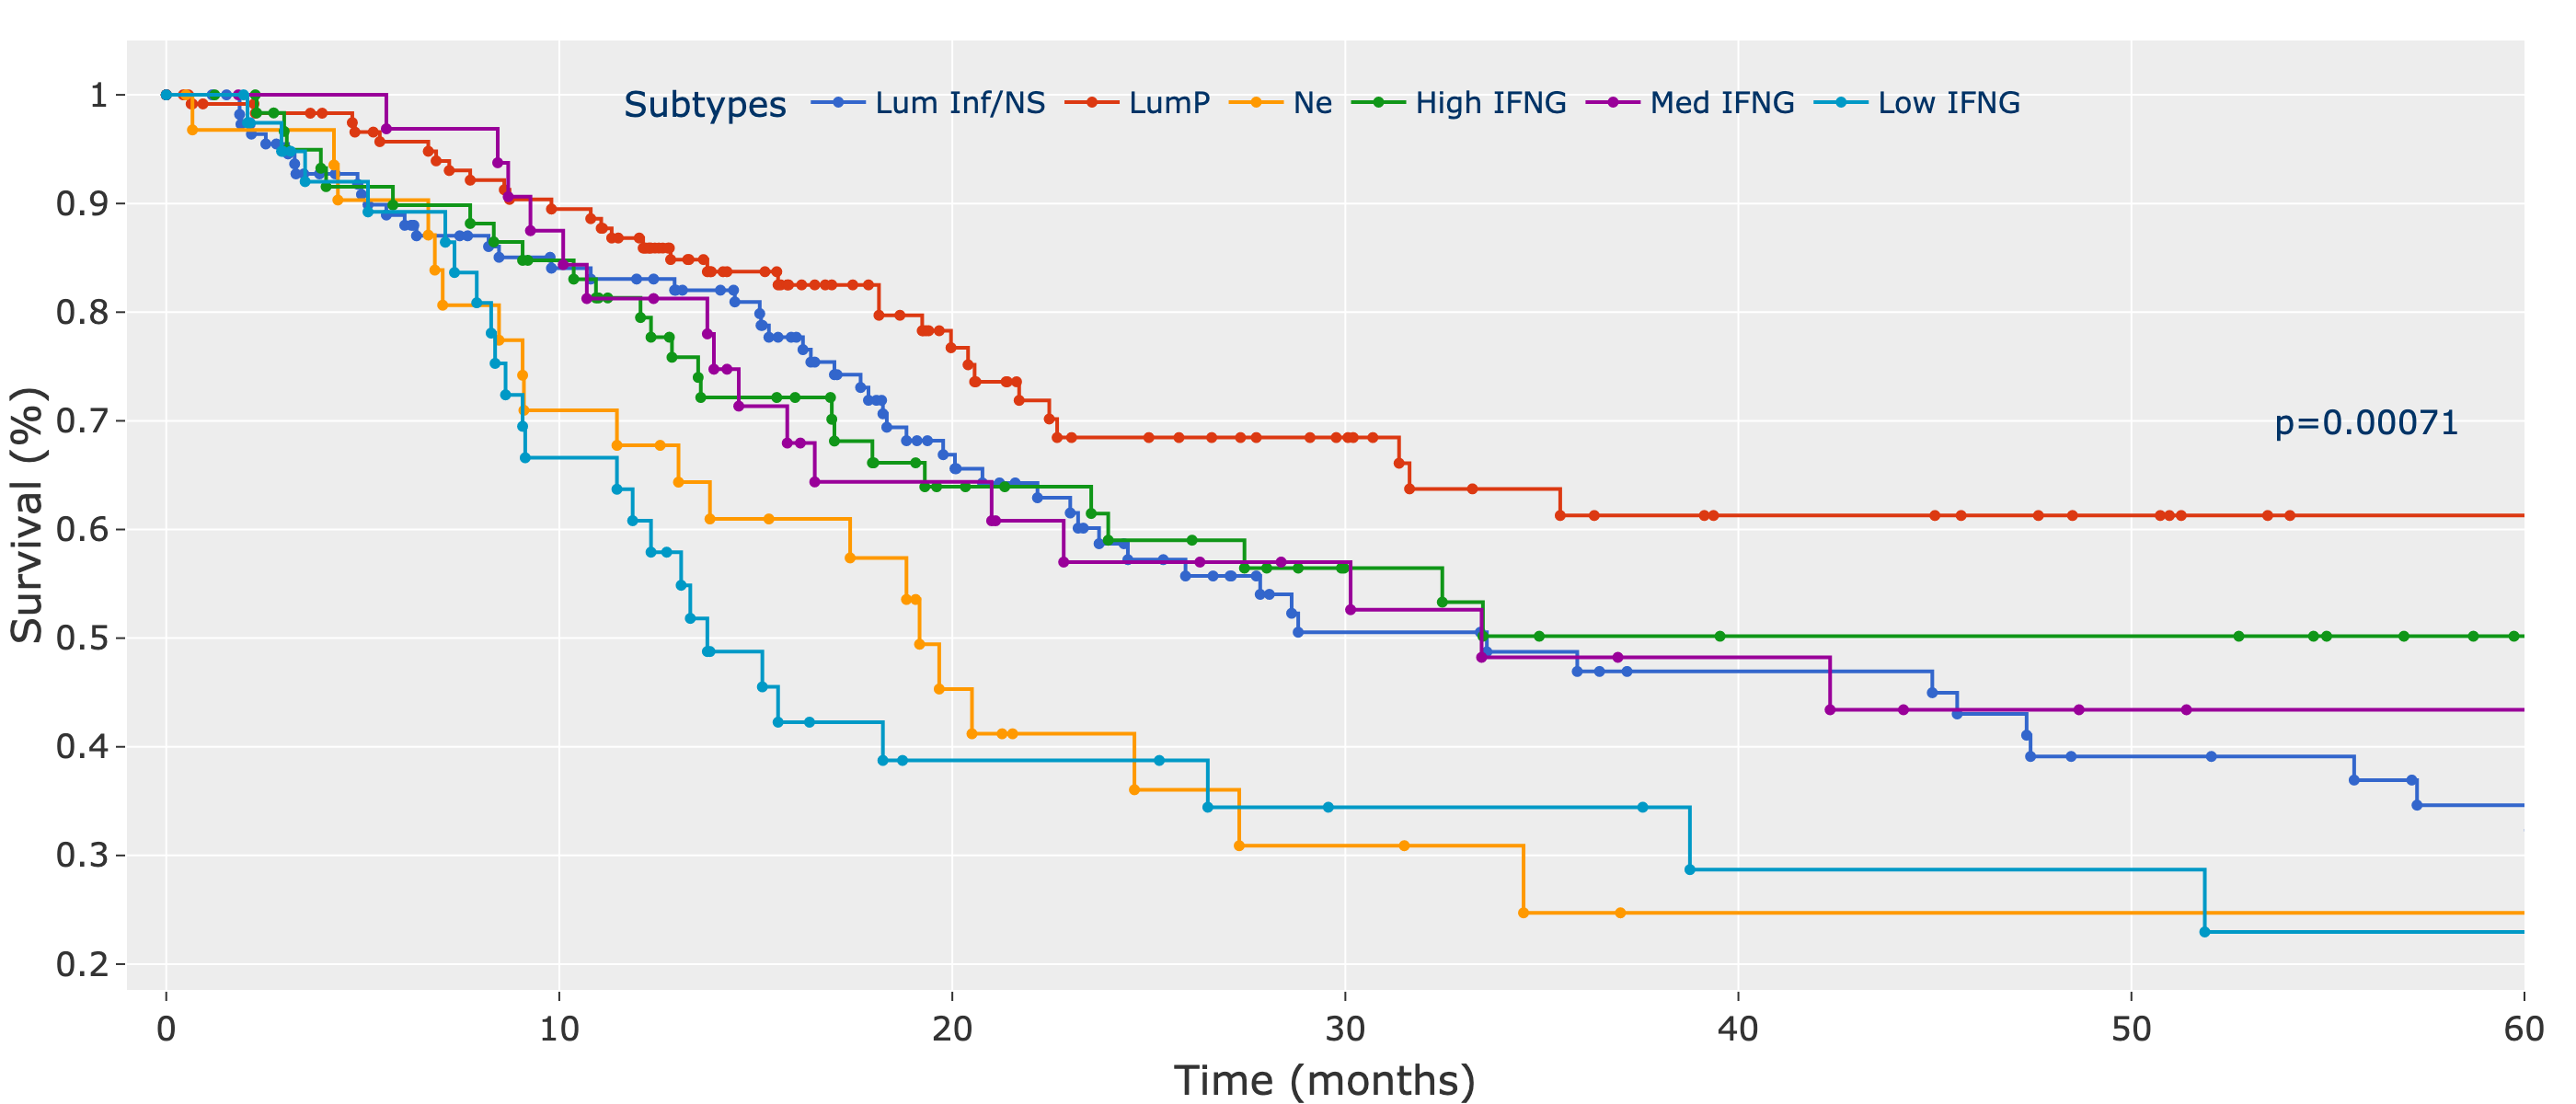
\includegraphics[width=\textwidth,keepaspectratio]{Sections/ClusteringAnalysis/Resources/discussion/survival_K_6.png}    
        \caption{Survival Kaplan-Meier}
        \label{fig:cs:survail_K}
    \end{subfigure}
    \centering
    \begin{subfigure}[!t]{1.0\textwidth}
        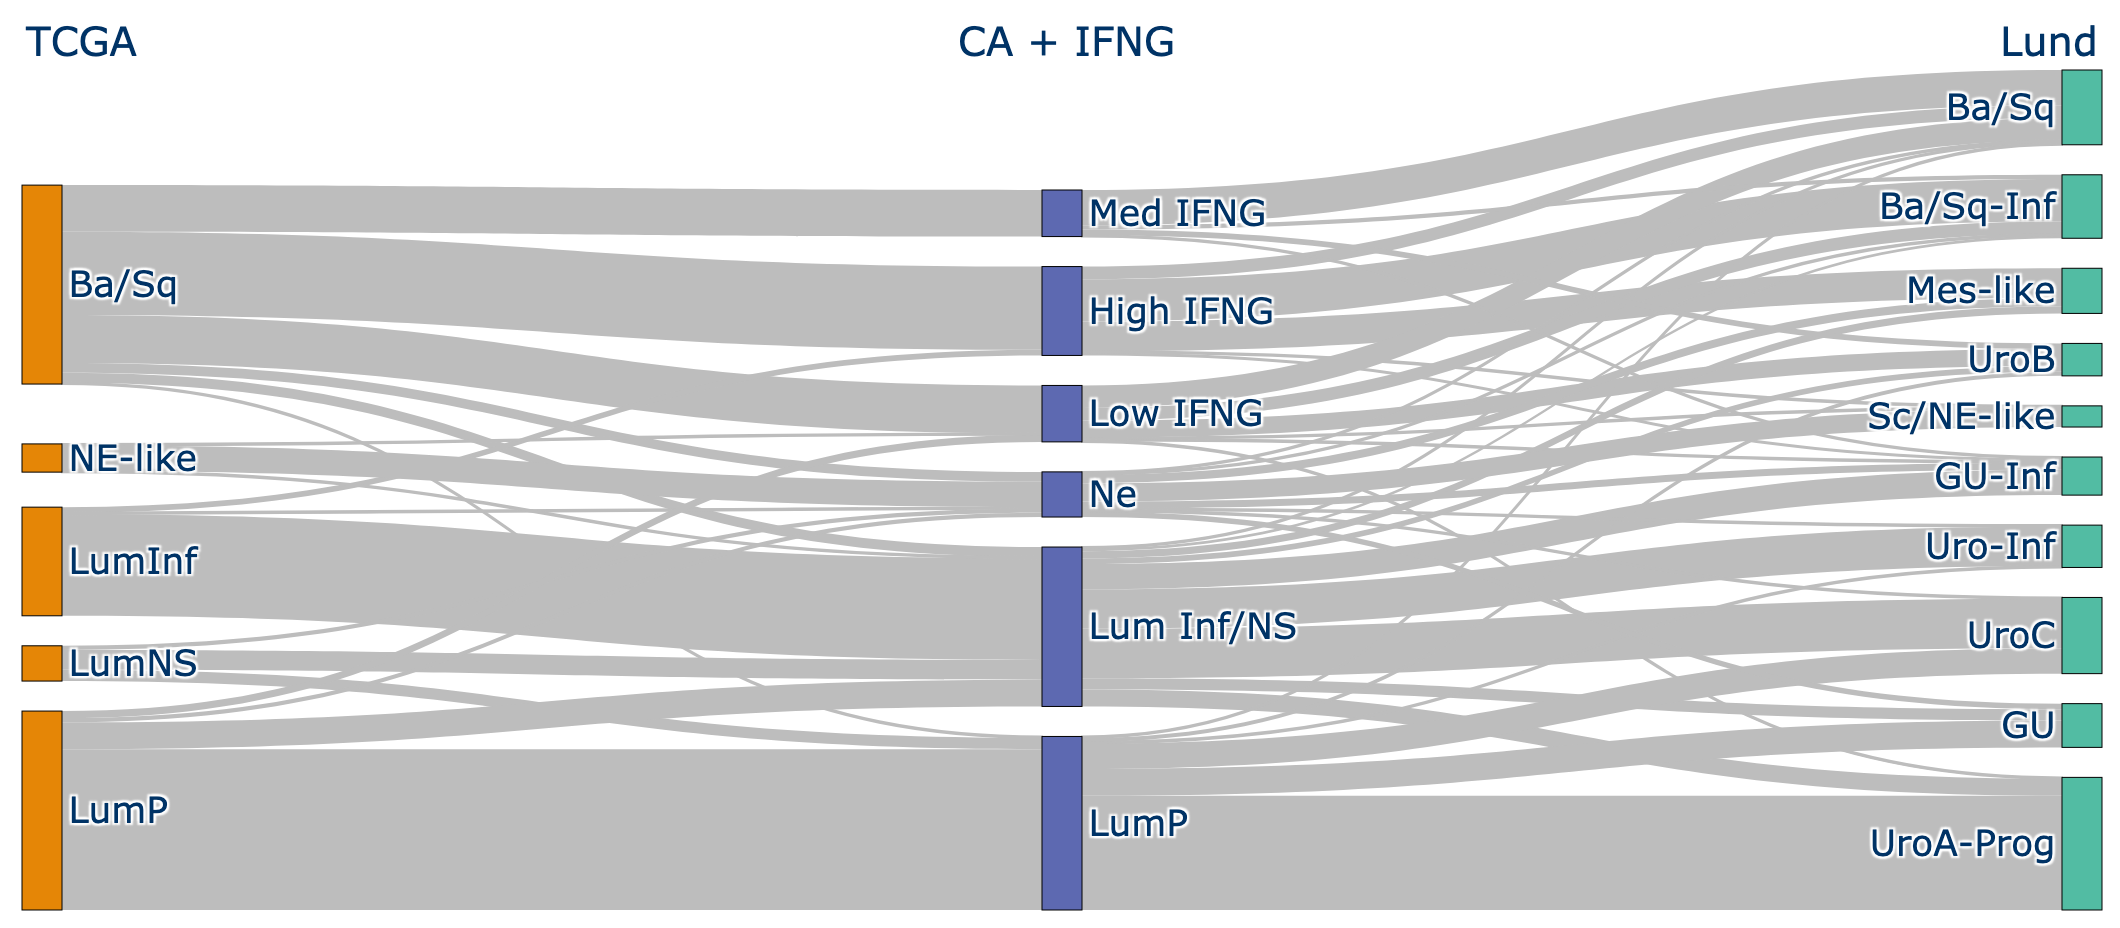
\includegraphics[width=\textwidth,keepaspectratio]{Sections/ClusteringAnalysis/Resources/discussion/KMeans_6_comp.png}
        \caption{Sankey plot}
        \label{fig:cs:stroma_basal}
    \end{subfigure} 
    \centering
    \caption{Overview of the MIBC subtypes derived from using K-means K=5 and the \acrshort{ifn} Basal stratification form \citet{Baker2022-bj}. The first plot shows the Kaplan-Meier survival analysis of the 6 subgroups find, Ne and Low IFNG having the poorest prognosis. The Sankey at the bottom shows how the subtypes found are compared with the TCGA \citet{Robertson2017-mg} and Lund \citet{Marzouka2018-ge} classifiers.} 
    \label{fig:cs:overview_K_means_6}
\end{figure}


\newpage

\begin{todolist}
    \item VU vs Robertson vs Consensus - done
    \item VU vs Lund - done
    \item VU vs SB - done
    \item DEA: Two basal splits - done
    \item DEA: Basal vs Luminal - done
    \item DEA: Compare with SB's changes - done
    \item DEA: Compare the splits in the larger Basal from VU - done
    \item Looking at the score in the metadata. Is there any correlation between the 
    \item Clustertree - done
    \item Survival analysis. Comparison between Basal subgroups.
    \item Gene Signature Enrichment Analysis (GSEA) on the different groups 
\end{todolist}
